%% Copyright 2019 Matheus H. J. Saldanha <mhjsaldanha@gmail.com>
%
% This work may be distributed and/or modified under the
% conditions of the LaTeX Project Public License, either version 1.3
% of this license or (at your option) any later version.
% The latest version of this license is in
%   http://www.latex-project.org/lppl.txt
% and version 1.3 or later is part of all distributions of LaTeX
% version 2005/12/01 or later.
%
% This work has the LPPL maintenance status `maintained'.

\documentclass[12pt,a4paper]{article}

% Pacotes para o português.
\usepackage[english]{babel}
\usepackage[utf8]{inputenc}
\usepackage[T1]{fontenc}

\usepackage{graphicx}     % Comando \includegraphics
\usepackage{xcolor}       % Comando de cores \textcolor
\usepackage{indentfirst}  % Indenta o primeiro parágrafo de cada seção
\usepackage{url}          % Comandos \url e \href
\usepackage[top=2cm, bottom=2cm, left=2cm, right=2cm]{geometry} % Define as margens do documento
\usepackage{multirow}     % Permite criar tabelas com uma célula ocupando várias linhas
\usepackage{amssymb}      % Símbolos matemáticos
\usepackage{amsmath}      % Ambientes para escrever fórmulas, \begin{align} por exemplo.
\usepackage{caption}      % Para definir o estilo das legendas de figuras e tabelas.
\usepackage{setspace}     % Para definir espaçamento entre linhas. (\onehalfspacing, \singlespacing, \doublespacing)
\usepackage{breakcites}   % Para permitir quebra de linha no meio de citações.
%\usepackage{times}        % Fonte Times New Roman
\usepackage{lipsum}       % Para gerar texto temporário. Exemplo: \lipsum \lipsum[1] \lipsum[4-5].
\usepackage{inconsolata}  % Fonte boa para códigos e URLs. Use \texttt{}
\usepackage{hyperref}     % Faz os links ficarem azuis e clicáveis. Facilita a navegação pelo PDF.

\makeatletter
\hypersetup{
	pdfkeywords={research project},
	colorlinks=true,       		% false: boxed links; true: colored links
	linkcolor=blue,          	% color of internal links
	citecolor=blue,        		% color of links to bibliography
	filecolor=magenta,      	% color of file links
	urlcolor=blue,
	bookmarksdepth=4,
}
\makeatother

\makeatletter
\renewcommand\tableofcontents{%         % Redefine table of contents to our taste
    \section*{\huge\centering\contentsname
        \@mkboth{%
           \MakeUppercase\contentsname}{\MakeUppercase\contentsname}}%
           \vspace{24pt}%
    \@starttoc{toc}%
    \newpage%
}

% Comando para marcar o texto para revisão.
\newcommand{\rev}[1]{\textcolor{red}{#1}}

% Permite escrever aspas normais "text" em vez de ``text''
\usepackage[autostyle]{csquotes}
\MakeOuterQuote{"}


\newcommand\underrel[2]{\mathrel{\mathop{#2}\limits_{#1}}}

\newcommand{\matriz}[1]{\hat#1}

\newcommand{\many}[2]{$#1_1, #1_2, \dots, #1_#2$}

\newcommand{\cmany}[3]{$#1_1 #3 #1_2 #3 \dots #3 #1_#2$}

\newcommand{\mmany}[2]{ #1_1, #1_2, \dots, #1_#2 }

\newcommand{\mcmany}[3]{#1_1 #3 #1_2 #3 \dots #3 #1_#2}

\newcommand{\set}[1]{\{#1\}}

\newcommand{\cjgt}[1]{\overline{#1}}
\DeclareMathOperator{\diag}{diag}
\DeclareMathOperator{\sign}{sign}
\DeclareMathOperator{\ai}{Ai}
\DeclareMathOperator{\re}{Re}
\DeclareMathOperator{\im}{Im}
\DeclareMathOperator{\Df}{D}
\DeclareMathOperator{\Ee}{E}
\DeclareMathOperator{\h}{h_1}
\DeclareMathOperator{\f}{f}
\DeclareMathOperator{\U}{U}
\DeclareMathOperator{\W}{W}
\DeclareMathOperator{\K}{K}
\DeclareMathOperator{\Hf}{\mathcal{H}}
\DeclareMathOperator{\Qf}{Q}
\DeclareMathOperator{\Gl}{\mathcal{L}}
\DeclareMathOperator{\g}{g}
\DeclareMathOperator{\V}{V}
\DeclareMathOperator{\Glin}{GL}
\newcommand{\iu}{\mathrm{i}\mkern1mu}
\renewcommand{\Im}{\mathop{\textrm Im}}
\DeclareMathOperator{\ee}{e}
\DeclareMathOperator{\supp}{supp}
\newcommand{\N}{\mathbb{N}}
\newcommand{\C}{\mathbb{C}}
\newcommand{\R}{\mathbb{R}}
\newcommand{\Z}{\mathbb{Z}}
\newcommand{\D}{\mathbb{D}}
\newcommand{\Q}{\mathbb{Q}}
\newcommand{\J}{J} %Jacobiano
\newcommand{\Id}{\mathbb{1}}
\newcommand{\p}{p} %medida
\newcommand{\E}{\mathbb{E}}
\newcommand{\Se}{\mathbb{S}}
\newcommand{\He}{\mathbb{H}}
\newcommand{\boh}{\mathit{o}}
\newcommand{\Boh}{\mathcal{O}}
\newcommand{\bbp}{\bm K_{\mathrm{BBP}}}
\newcommand{\ii}{\mathrm{i}}
\newcommand*{\deff}{\mathrel{\vcenter{\baselineskip0.5ex \lineskiplimit0pt
			\hbox{\scriptsize.}\hbox{\scriptsize.}}}%
	=}
\newcommand*{\revdeff}{=\mathrel{\vcenter{\baselineskip0.5ex \lineskiplimit0pt
			\hbox{\scriptsize.}\hbox{\scriptsize.}}}%
}


% MATH DECLARATIONS
\newtheorem{lemma}{Lema}[section]
\newtheorem{thm}[lemma]{Teorema}
\newtheorem{claim}[lemma]{Afirmação}
\newtheorem{cor}[lemma]{Corolário}
\newtheorem{definition}[lemma]{Definição}
\newtheorem{conjecture}[lemma]{Conjectura}
\newtheorem{prop}[lemma]{Proposição}
\newtheorem{assumption}[lemma]{Assumpção}
\numberwithin{equation}{section} %numeracao dentro de secoes

% PROOF ENV
\makeatletter
\newenvironment{proof}[1][Demonstração]{\par
	\pushQED{\qed}%
	\normalfont \topsep6\p@\@plus6\p@\relax
	\trivlist
	\item\relax
	{\itshape
		#1\@addpunct{.}}\hspace\labelsep\ignorespaces
}{%
	\popQED\endtrivlist\@endpefalse
}
\makeatother
\newcommand{\dd}{\mathrm{d}}
%%%%%

\begin{document}

\doublespacing

\begin{titlepage}
    \begin{center}
        {\large \sc Universidade de São Paulo} \\
        {\large \sc Fundação de Amparo à Pesquisa do Estado de São Paulo}\\
        {\large \sc Proposta de Projeto de Mestrado A}
        
        \vspace{1cm}

        % % Título.
        {\Large \bfseries Assintóticas de Funções Partição em Gases de Coulomb} \\
        \vspace{1cm}
		{\small \sc Proposta vinculada ao Projeto Jovem Pesquisador entitulado} \\
		{\small \sc Análise Assintótica de Sistemas de Partículas e Matrizes Aleatórias} \\
		\vspace{1cm}

        % % Participantes
        {\small \sc \textbf{Proponente/beneficiário}: João Victor Alcantara Pimenta}\\
        {\small \sc \textbf{Orientador:} Guilherme L. F. Silva}\\[0.5cm]
        
        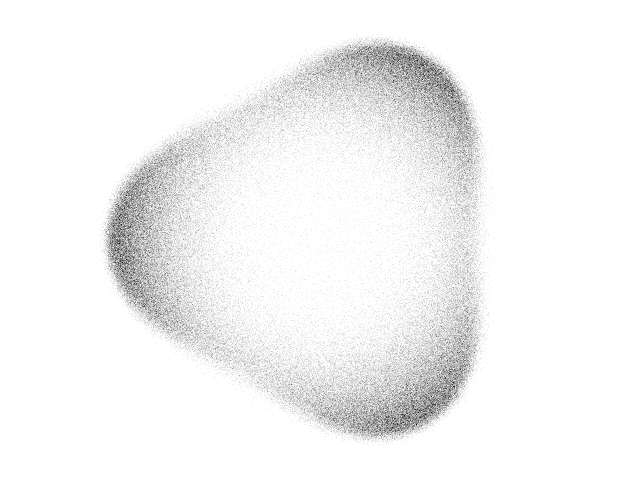
\includegraphics[scale=0.30]{Assets/CuteCircleWhite2}
        
    \end{center}

    \vfill

    \begin{center}
        {\bf \large Resumo} \\[1em]
    \end{center}
    O estudo de Matrizes Aleatórias demonstra aplicabilidade em uma gama diversa de áreas na matemática e na física, com destaque no estudo de mecânica estatística. No estudo da medida do espectro de autovalores de alguns ensembles de matrizes, analogias físicas à sistemas termodinâmicos se tornam evidentes e algumas motivações físicas podem ser tomadas. Um exemplo disso é a descrição da função partição, que em termodinâmica guarda grande detalhe sobre o sistema e suas propriedades. Desenvolvimentos recentes tem progredido intensamente na expressão para a expansão, no limite termodinâmico, da função partição de alguns sistemas termodinâmicos compatíveis com ensembles de interesse. O objetivo deste trabalho é estudar tais desenvolvimentos e entender suas implicações e importância dentro da teoria de matrizes aleatórias.

    % Data
    % \begin{center}
    %     \makeatletter
    %     São Carlos, SP \\
    %     \@date
    %     \makeatother
    % \end{center}
    
\end{titlepage}

\begin{titlepage}
    \begin{center}
        {\large \sc University of São Paulo} \\
		{\large \sc São Paulo Research Foundation}\\
    	{\large \sc Proposal of Masters Project A}
    	
    	\vspace{1cm}
    	
    	% % Título.
    	{\Large \bfseries Asymptotics of Partition Functions on Coulomb Gases} \\
    	\vspace{1cm}
    	{\small \sc Proposal vinculated to the "Jovem Pesquisador" research proposal entitled} \\
    	{\small \sc Asymptotic Analysis of Interacting Particle Systems and Random Matrix Theory} \\
    	\vspace{1cm}
    	
    	% % Participantes
    	{\small \sc \textbf{Principal Investigator/beneficiary}: João Victor Alcantara Pimenta}\\
    	{\small \sc \textbf{Supervisor:} Guilherme L. F. Silva}\\[0.5cm]
    	
    	
\includegraphics[scale=0.35]{Assets/CuteCircleWhite}
    	
    \end{center}

    \vfill

    \begin{center}
        {\bf \large Abstract} \\[1em]
    \end{center}
    The study of Random Matrices demonstrates applicability in a diverse range of areas in mathematics and Physics, emphasizing the study of statistical mechanics. In the study of the spectra of eigenvalue on some random matrices ensembles, an physical analogy regarding thermodynamical systems becomes evident and the use of physical motivations in its study of great importance. An example of such motivation is the study of the partition function, witch holds in thermodynamics a great deal of information on the system as hand and its properties. Recent developments have been intensely changing what is know on the thermodynamical limit asymptotic of these partition functions, especially for systems that regard ensembles of matrices of interest in modern research. The main goal of this work is to understand this developments and its implication and importance in the theory of random matrices.

    
\end{titlepage}


% \noindent{}
% \newpage
% \pagestyle{empty} % Não numera a página
% \tableofcontents
% \newpage
\setcounter{page}{1}
\pagestyle{plain} % Agora passa a numerar as páginas

\section{Introduction}
\label{section:introducao}
A random matrix is a matrix in which the entries are random variables, not necessarily independent nor equally distributed. The algebraic-geometric properties in a matrix, such as its natural multiplication and spectral decomposition, makes this representation especially useful. Naturally, many complex systems use a matrix representation. Correlation matrices and operators, especially in physics, are some of many major reasons why this representation is important. Studying these matrices we can deduce properties from the system of interest, either that being the eigenvalues and eigenvectors of operators describing an atomic nuclei \cite{Dyson} or the description of market shares in highly correlated systems \cite[Chapter~2]{fabozziquantitative}. Either way, using an random matrix approach is relevant by the same reason random variables proved themselves crucial: it unlocks relevant statistical description of phenomena and systems.

In the research proposed here, we will focus on the study of {\it normal random matrices}, which consists of the space of normal matrices, equipped with a proper probability distribution. In our case, such probability distribution is given by a Gibbs-type measure, which we also impose to be invariant under the action of the unitary group. All in all, such invariance imposes a trivialization of the eigenvectors, which turn out to be simply Haar-distributed on the unitary group. In turn, all the relevant information on the matrix model is contained in their eigenvalues, and their joint probability density function is explicitly given by
%
\begin{equation}
		\p(\mmany{\lambda}{N}) = \frac{1}{Z_{N, \beta}} \ee^{-\beta_N \mathcal{H}_N(\vec{\lambda})},\quad (\lambda_1,\hdots,\lambda_N)\in \mathbb C^N
	\label{Equation: Gaussian measure}
\end{equation}
where $Z_{N, \beta}$ is the canonical partition function, such that $\p$ is a probability density with respect to the Lebesgue measure on $\mathbb C^N$. The factor $\beta_N = \beta N^2$ is though of as the inverse temperature and the factor $\mathcal H_N$, called the Hamiltonian, is given by
%
$$\mathcal{H}_N(\vec{\lambda}) = \frac{1}{N}\sum_{i = 1}^{N} V(\lambda_i) + \frac{1}{N^2} \sum_{i < j} \log{\frac{1}{|\lambda_i - \lambda_j|}}, \quad (\lambda_1,\hdots,\lambda_N)\in \mathbb C^N$$
%
where $V:\mathbb C\to \mathbb C$ is a suitably regular function, acting as a confining potential on the eigenvalues $\lambda_1,\hdots, \lambda_N$. 

Considering such a measure is natural to make an analogy to the well know Coulomb Gas. Under appropriate conditions, the Coulomb Gas is a Gibbs-Boltzmann probability measure given in $(\mathbb R^d)^N$. This measure $\p_N$ models an interacting gas of charged particles, at $\mmany{x}{N} \in \Se$ of dimension $d$ in $\R^n$ ambient space, under the influence of an external potential. Its measure its given by 
\begin{equation}
	\p_N(\mmany{x}{N}) = \frac{e^{-\beta N^2 \Hf_N(\mmany{x}{N})}}{Z_{N,\beta}},
	\label{Equação: Medida Gas de Coulomb}
\end{equation}
where $$\Hf_N(\vec{x}) = \frac{1}{N} \sum_{i = 1}^{N} \V(x) + \frac{1}{2N^2} \sum_{i \neq j} \g(x_i - x_j)$$ is the Hamiltonian or energy of the system and $\g(x_i - x_j)$ is the Coulomb Kernel of interaction. In this analogy, eigenvalues $\lambda_1,\hdots, \lambda_N$ may be seen as particles under the influence of the Gibbs law, and thermodynamical arguments may be employed to describe the configurations of eigenvalues of random matrices. With this in mind we turn to the partition function. In the beginning of its book, Feynman states \cite{feynmanstatistical} that the key principle of the statistical mechanics is that the probability that a system attains a state with energy $E$, in equilibrium, is given by a function $\frac{1}{Z} \ee^{\frac{-E}{kT}}$ where $Z$ is the partition function. In a more general sense there is a relation between the partition function and the free energy of the system, that, in itself, relates to the entropy. Knowing well the partition function is a way to describe with great detail the macro-properties of such a system.

There is a great effort in the community of random matrix theory to study expansions of the partition function of systems such of Coulomb Gases. Recently, some advance has been made in the works of Sug-Soo Byun et al. \cite{Byun_2023}. They derived large-$N$ asymptotic expansions up to the $O(1)$-terms for  $Z_{N,\beta}$ when $V$ is a radially symmetric potential, in the form
%
$$
Z_{N,\beta=2}=-I^VN^2+\frac{1}{2}N\log N+E^V N+G\log N+F^V + o(1),\quad N\to \infty.
$$
%
In such expansion, for a large class of potentials $V$ the first term $I^Q$ was known for a long time, being given by the energy of the associated equilibrium measure. The coefficient $1/2$ of the order $N\log N$, as well as the entropy term $E^V$, were known from recent work of Leblé and Serfaty \cite{leblé2017large}, also for rather large classes of $V$. The remaining terms in this expansion are new, and they are computed exploring the radially symmetry imposed on the potential. Strikingly, the term $G$ appears to be universal in $V$, depending solely on the connectivity of the limiting spectrum of eigenvalues. More precisely, they noticed that $G$ depends on whether the limiting spectrum is an annulus or a disc which, surprisingly, seems to not have been observed in the vast previous literature on the matter. 

As was said, the study of the partition function is a major way to describe thermodynamical systems such that of a Coulomb Gas. With these new developments it is expected that many systems could be better understood and described by the asymptotic given. In that way this poses a great opportunity for development in the field. More than that, by the great connection that the field of random matrices holds with many other fields is possible that by the study of this work some suggestions on the behavior of many other related problems become plausible.


\section{Main Goals and Methodology}
\label{section:objetivos}
This MD research proposal has ? main goals.....


\begin{enumerate}
	\item \textbf{Goal 1};
	
	\item \textbf{Goal 2};
	
	\item \textbf{Goal 3};
	
	\item \textbf{Goal 4};
	
\end{enumerate}

\section{Necessary Background}
\label{section:Materiais&Metodos}
This project requires some knowledge in a few mathematical areas. Some of them are real and complex analysis, functional analysis, measure theory and correlated courses. All of those are provided at the necessary leal ate the Masters Program in Mathematics at the ICMC - USP. All required background is expected to be gained in the regular courses in the first terms of the program, as usual. Some other disciplines may be coursed during the summer courses at the same institute. Furthermore, te student has had a year of experience in Random Matrix Theory at an undergrad level within a FAPESP fellowship supervised by the same researcher in witch some experience and general knowledge of the field has been gained.

\section{Brief Schedule}
\label{section:Planos&Cronograma}

This M.D. research proposal is schedule to start at August 2024 and run for te usual time for the Masters Program, that is, 24 months. The project will be run with weekly meetings with the supervisor, and sporadic seminar expositions to the other members of the research team associated with the JP Research Grant and correlated groups. We can divide the project executions in the following schedule. The steps are as described in Section \ref{section:objetivos}.

\begin{table}[ht]
\centering
\begin{tabular}{|c|c|c|c|c|c|c|c|c|c|c|c|c|}
\hline
\multirow{2}{*}{{\bf Steps}} & \multicolumn{8}{c|}{{\bf Quarters}}
\\ \cline{2-9}
    & 1 & 2 & 3 & 4 & 5 & 6 & 7 & 8
\\ \hline
    {\bf 1. Master Courses} & \textcolor{red}{x} & \textcolor{red}{x} & \textcolor{red}{x} & \textcolor{red}{x} & x & x & & 
\\ \hline
    {\bf 2. Concepts} &  &  & x & \textcolor{red}{x} & \textcolor{red}{x} & x & &
\\ \hline
    {\bf 3. Main Article} & & & & x & \textcolor{red}{x} & \textcolor{red}{x} & x &
\\ \hline
    {\bf 4. Exploration} & & & & & x & \textcolor{red}{x} & \textcolor{red}{x} & 
\\ \hline
    {\bf 5. Masther Thesis} & & & & & x & \textcolor{red}{x} & \textcolor{red}{x} & \textcolor{red}{x}
\\ \hline
\end{tabular}
\caption{Activities planning, te steps are as described in th Section \ref{section:objetivos}. Red color indicates the focus of the quarter that may be divided between activities for some crucial quarters.}
\label{tab:cronograma1ano}
\end{table}

\bibliographystyle{apalike}
\bibliography{bibliography.bib}

\end{document}